\documentclass{article}

% Language setting
% Replace `english' with e.g. `spanish' to change the document language
\usepackage[english]{babel}

% Set page size and margins
% Replace `letterpaper' with `a4paper' for UK/EU standard size
\usepackage[letterpaper,top=2cm,bottom=2cm,left=3cm,right=3cm,marginparwidth=1.75cm]{geometry}

% Useful packages
\usepackage{amsmath}
\usepackage{graphicx}
\usepackage[colorlinks=true, allcolors=blue]{hyperref}
\usepackage{listings}
\lstset{language=R,
    basicstyle=\small\ttfamily,
    stringstyle=\color{DarkGreen},
    deletekeywords={I, df, aov},
    keywordstyle=\color{blue},
    commentstyle=\color{DarkGreen},
    numbersep=8pt
}
\usepackage{enumitem}
\renewcommand\thesubsection{\Alph{subsection}}

\title{Report 1}
\author{You}

\begin{document}
\maketitle

\begin{abstract}
Your abstract.
\end{abstract}

\section{Ice cream}

\section{Hemoglobin in trout}

\begin{figure}[h]
    \centering
    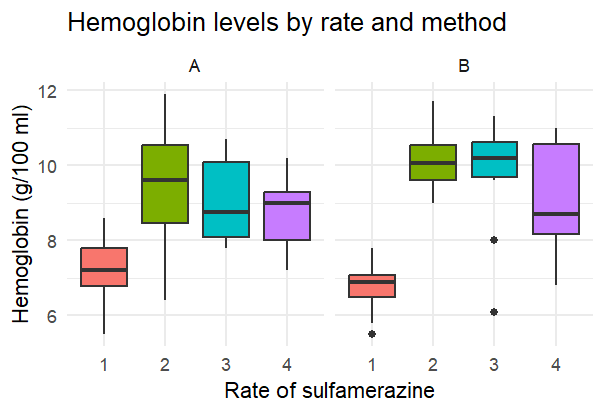
\includegraphics[height=5cm]{BoxplotHemoglobin.png}
    \caption{This boxplot illustrates the variation of hemoglobin levels across different rates of sulfamerazine, categorized by two different methods (A and B). Rates are defined as 0, 5, 10 and 15 grams of sulfamerazine per 100 pounds of fish. The rate of 1, indicating no sulfamerazine, is associated with lower hemoglobin levels compared to higher rates. }
    \label{fig:boxHem}
\end{figure}

\subsection{Randomization in R}
\begin{lstlisting}[caption="Randomization in R",label={lst:R}]
    rbind(rep(1:I, each = N * J), rep(1:J, N*I), sample(1:(N*I*J)))
\end{lstlisting}

\subsection{Two-way ANOVA}
\begin{lstlisting}[caption="Two-way ANOVA", label={lst:T}]
    hemoglobin_df$rate <- as.factor(hemoglobin_df$rate) 
    hemoglobin_df$method <- as.factor(hemoglobin_df$method)
    hemoglobin_aov <- lm(hemoglobin ~ rate*method, data = hemoglobin_df)
    anova(hemoglobin_aov)   
\end{lstlisting}

\begin{table}[ht]
\centering
\caption{Two-way ANOVA Table for Hemoglobin Levels by Rate and Method} 
\label{tab:hemoglobin_anova}
\begin{tabular}{lrrrrr}
  \hline
 & Df & Sum Sq & Mean Sq & F value & Pr($>$F) \\ 
  \hline
rate & 3 & 90.56 & 30.19 & 19.47 & 0.0000 \\ 
  method & 1 & 2.42 & 2.42 & 1.56 & 0.2161 \\ 
  rate:method & 3 & 4.87 & 1.62 & 1.05 & 0.3769 \\ 
  Residuals & 72 & 111.64 & 1.55 &  &  \\ 
   \hline
\end{tabular}
\end{table}

The p value for testing H0: $\alpha_i$ = 0 for all i is 2.404e-09. 
Therefore, we reject the null hypothesis and conclude that the rate of sulfamerazine is not the same for all methods.

The p value for testing H0: $\beta_j$ = 0 for all j is 0.2161.
Therefore, we fail to reject the null hypothesis and conclude that the two methods for different types sulfamerazine is the same for all rates of sulfamerazine.

The p value for testing H0: $\gamma_{i*j}$ = 0 for all (i, j) is 0.3769.
So, there is no evidence for interaction.
\begin{table}[ht]
\caption{Treatment Parameterization in ANOVA}
\label{tab:treatment}
\centering
\begin{tabular}{rrrrr}
  \hline
 & Estimate & Std. Error & t value & Pr($>$$|$t$|$) \\ 
  \hline
(Intercept) & 7.2000 & 0.3938 & 18.28 & 0.0000 \\ 
  rate2 & 2.1300 & 0.5569 & 3.82 & 0.0003 \\ 
  rate3 & 1.8300 & 0.5569 & 3.29 & 0.0016 \\ 
  rate4 & 1.4900 & 0.5569 & 2.68 & 0.0092 \\ 
  methodB & -0.4500 & 0.5569 & -0.81 & 0.4217 \\ 
  rate2:methodB & 1.2600 & 0.7875 & 1.60 & 0.1140 \\ 
  rate3:methodB & 1.1500 & 0.7875 & 1.46 & 0.1486 \\ 
  rate4:methodB & 0.7800 & 0.7875 & 0.99 & 0.3253 \\ 
   \hline
\end{tabular}
\end{table}

\subsection{Additive model}
\begin{lstlisting}[caption="Additive model for Two-Way ANOVA", label={lst:Add}]
    hemoglobin_aov_2 <- lm(hemoglobin ~ rate+method, data = hemoglobin_df)
    anova(hemoglobin_aov_2) 
\end{lstlisting}


\subsection{One-way ANOVA}

\subsection{Kruskal-Wallis test}


\section{Exercise 3}


\bibliographystyle{alpha}
\bibliography{sample}

\end{document}